\section{Macroeconometric analysis}\label{sec:VECM}

\subsection{Houses' own interest rate and residential investment growth rate in the US	Economy}\label{sec:own}

This subsection aims to describe the relationship between residential investment growth rate ($g_{I_h}$) and houses' own interest rate ($own$) proposed by \textcite{teixeira_crescimento_2015}. 
Next, we will present the hypothesis to be tested on the Section \ref{sec:estimation}. To demonstrate this relationship, the mortgage interest rate ($r_{mo}$) is deflated by the real estate inflation ($\pi$) as follows:

$$
g_{I_h} = \phi_0 - \phi_1\cdot \overbrace{\left(\frac{1+r_{mo}}{1+\pi} - 1\right)}^{own}
$$


\begin{equation}
g_{I_h} = \phi_0 - \phi_1\cdot own
\end{equation}
where $\phi_0$ represents long-term determinants (\textit{e.g.} demographic factors, housing and credit policies, etc.) while $\phi_1$ captures the demand for real estate arising from expectations of capital gains resulting from speculation with the existing dwellings stock. 

This particular real interest rate is the most relevant for households since the holders of an asset take their price into account in the decision-making process since its variation can generate capital gains/losses (\cite[p.~114]{teixeira_crescimento_2015}).
In other words, the mortgage interest rate captures debt service for investors --- in this case, households --- while the real estate inflation allows incorporating changes in equity. Therefore, this own interest rate stands for the real cost in real estate from buying real estate  (\cite[p.~53]{teixeira_crescimento_2015}).

Figure FIGURE shows how this deflation procedure is more adequate than a general price index --- as \textcite[p.~143--6]{fair_macroeconometric_2013} does --- to describe the housing dynamics. It worth noting that during a houses' bubble period, it is real estate inflation that governs own's interest rate dynamics.
Therefore, the lower this rate is, the greater the capital gains (in real estate) for speculating with real estate will be. This negative relation between houses' own interest rate and residential investment is shown in Figure FIGURE in which this particular real interest rate has been gradually decreased over the real estate boom (2002-5).

Despite shedding light on some relevant relationships, \textcite{teixeira_crescimento_2015} proposition was not evaluated econometrically and this will be done in Section \ref{sec:estimation}. To do so, we assume the following long-run relationship:

\begin{equation}
g_{I_ht} = \phi_0 - \phi_1\cdot own_t
\end{equation}
therefore, if these time-series are cointegrated, we model the short-run adjustment process through the following VECM:
\begin{equation}
\begin{cases}
\Delta own_t = \delta_{1} + \alpha_1\left(g_{I_{h_{t-1}}} - \phi_0 + \phi_1\cdot own_{t-1}\right) + {\sum^{N=4}_{i=1}}\beta_{1,i}\cdot \Delta g_{I_{h_{t-i}}} +
\sum^{N=4}_{i=1}\gamma_{1,i}\cdot \Delta own_{t-i} +\varepsilon_{t,1}
\\
\Delta g_{Z_{t}} = \delta_{2} + \alpha_2\left(g_{I_{h_{t-1}}} - \phi_0 + \phi_1\cdot own_{t-1}\right) + \sum^{N=4}_{i=1}\beta_{2,i}\cdot \Delta g_{I_{h_{t-i}}} +
\sum^{N=4}_{i=1}\gamma_{2,i}\cdot \Delta own_{t-i} +\varepsilon_{t,2}
\end{cases}
\end{equation}
where $\delta_s$ indicate linear trend in the series (level);
$\alpha_{is}$ are the error correction coefficients ; 
$\beta_s$ e $\gamma_s$ are coefficients associated with lagged $g_{I_h}$ and $own$ respectively and; $\varepsilon_s$ are the residual.
According to \textcite{teixeira_crescimento_2015}, the expected results are depicted in Table \ref{resultados_esperados} below:

% Please add the following required packages to your document preamble:
% \usepackage{graphicx}
\begin{table}[H]
	\centering
	\caption{Summary of expected results of the macroeconometric model}
	\label{resultados_esperados}
	\resizebox{\textwidth}{!}{%
		\begin{tabular}{l|l|l}
			\hline\hline
			\textbf{\begin{tabular}[c]{@{}l@{}}Expected\\ Result\end{tabular}} &
			\textbf{Econometric Meaning} &
			\textbf{Economic Meaning} \\ \hline\hline
			\textbf{1. $\varepsilon \sim I(0)$} &
			\begin{tabular}[c]{@{}l@{}} Stationary residuals indicates cointegration relationship\end{tabular} &
			\begin{tabular}[c]{@{}l@{}} Series share a common\\long-run trend\end{tabular} \\ \hline
			\textbf{2. $\alpha_1 = 0$} &
			\begin{tabular}[c]{@{}l@{}} $own$ is weakly exogenous\\ compered to $g_{I_h}$\end{tabular} & \begin{tabular}[c]{@{}l@{}} 
				$own$ dynamics is not affected\\by previous equilibrium deviation\end{tabular}
			\\ \hline
			\textbf{3. $\alpha_2 < 0$} &
			\begin{tabular}[c]{@{}l@{}}Own interest rate Granger-causes\\
				residential investment growth rate\end{tabular} & \begin{tabular}[c]{@{}l@{}} $g_{I_h}$ dynamics is not affected\\ by previous equilibrium deviation\end{tabular}
			\\ \hline
			\textbf{4. $\phi_1 > 0$} &
			\begin{tabular}[c]{@{}l@{}}Series share a common\\negative long-run relationship\end{tabular} &
			\begin{tabular}[c]{@{}l@{}}Own interest rate affects\\residential investment growth rate negatively\end{tabular} \\ \hline
			\textbf{5. $\phi_0 < 0$} &
			\begin{tabular}[c]{@{}l@{}}
			Real estate demand for non-speculation\\reasons is statistically significant
			\end{tabular} &
			\begin{tabular}[c]{@{}l@{}}
				Real estate demand associated with\\institutional particularities and demographic\\ changes affects residential investment\\growth rate positively\end{tabular} \\ \hline
			\textbf{6. $\gamma_{2,is} < 0$} &
			\begin{tabular}[c]{@{}l@{}}Residential investment growth rate\\coefficient is statistically significant\end{tabular} &
			\begin{tabular}[c]{@{}l@{}}Own interest rate affects\\$g_{I_h}$ in the short-run\end{tabular} \\ \hline
			\textbf{7. $\beta_{1,is} = 0$} &
			\begin{tabular}[c]{@{}l@{}}
				$g_{I_h}$ effects over own interest\\ rate is not statistically significant\end{tabular} &
			\begin{tabular}[c]{@{}l@{}}
				$g_{I_h}$ effects over own interest\\ rate is negligible since dwellings stock is much\\bigger than residential investment (flow)\end{tabular} \\ \hline\hline
		\end{tabular}%
	}
\caption*{\textbf{Source:} Authors' elaboration}
\end{table}



\subsection{Data and estimation strategy}\label{sec:estimation}

In this section, we employ a model to test if real estate inflation describes residential investment growth rate dynamics\footnote{Scripts are available under request.}. Our sample period (1992:Q1
to 2019:Q1) starts after institutional changes (FDIC e
FIRREA) due to the Savings and Loans crisis (see Table \ref{structbreak} in appendix \ref{appen:A} for some related structural breaks). 
We rely on the following  quarterly seasonally adjusted data: (i) 30-Year fixed mortgage interest rate (MORTGAGE30US, resampled by end of period), private residential investment (PRFI, growth rate as percent change from the previous quarter) and Case-Shiller home price index
(CSUSHPISA, resampled by end of period).

Next, we applied \textcite{yeo_new_2000} transformation since these series are quite volatile. The reason for using this procedure instead of \textcite{box_analysis_1964} transformation  it can be applied to non-positive values. 
Then, we employ standard unit root tests (see Table \ref{unitroot} in appendix \ref{appen:A}) as well as \textcite{johansen_estimation_1991} procedure to assess whether houses' own interest rate and residential investment growth rate share a common long-run trend (see Table \ref{Johansen} in appendix \ref{appen:A}).
Our series are cointegrated at 5\% significance level which allows us to estimate a error correction model and evaluate the previous hypothesis (\cite{enders_applied_2014}).

\begin{figure}[htb]
	\centering
	\caption{Time-series with \textcite{yeo_new_2000} transformation}
	\label{YeoJhonson}
	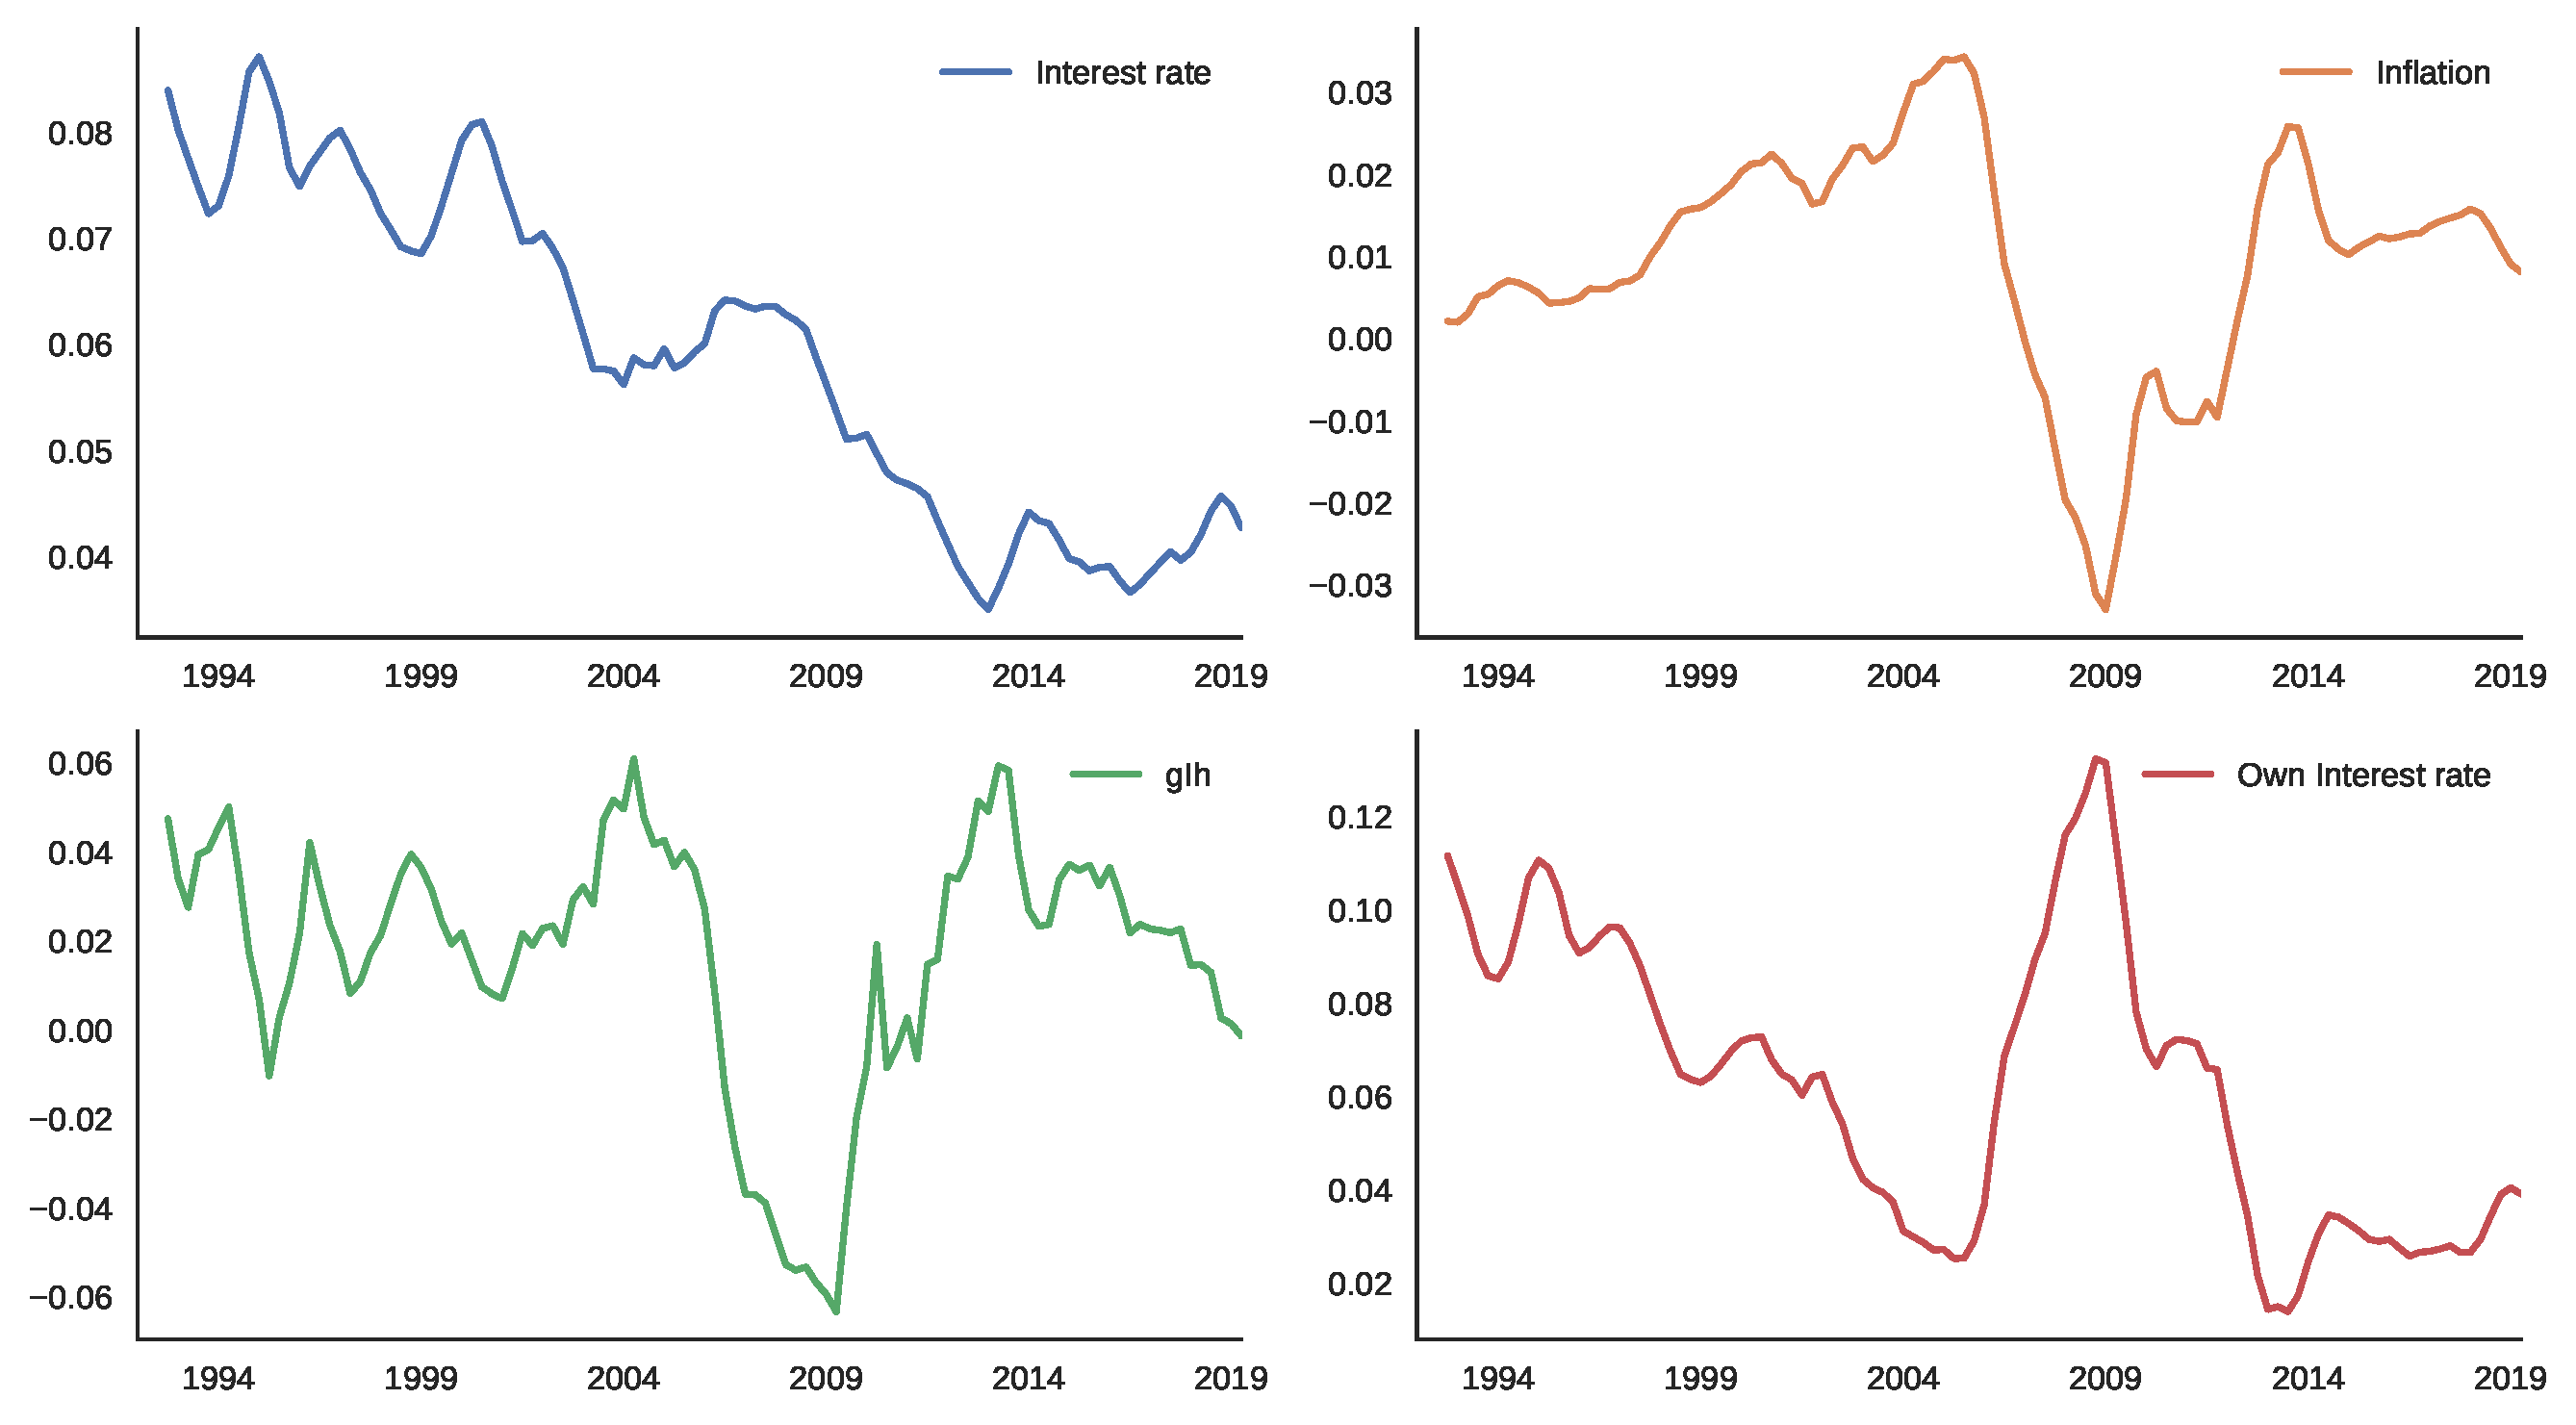
\includegraphics[width=\textwidth]{./figs/YeoJohnson_All}
	\caption*{\textbf{Source:} U.S. Bureau of Economic Analysis, Authors' elaboration}
\end{figure}


The next step is to define the order of lags. According to usual information criteria, both first and forth lags are eligible (see Table \ref{criterios} in appendix \ref{appen:A}).
Although parsimonious, the choice of the first lag has no empirical support.
Considering the average construction time (from approval to completion), we should include at least the second in order to incorporate homes built for capital gains purposes which only take place once the construction is completed (see Figure \ref{meses}).


\begin{figure}[H]
	\centering
	\caption{Average construction time (approval to completion) of properties for a family unit by construction purposes except manufactured houses (1976-2018)}
	\label{meses}
	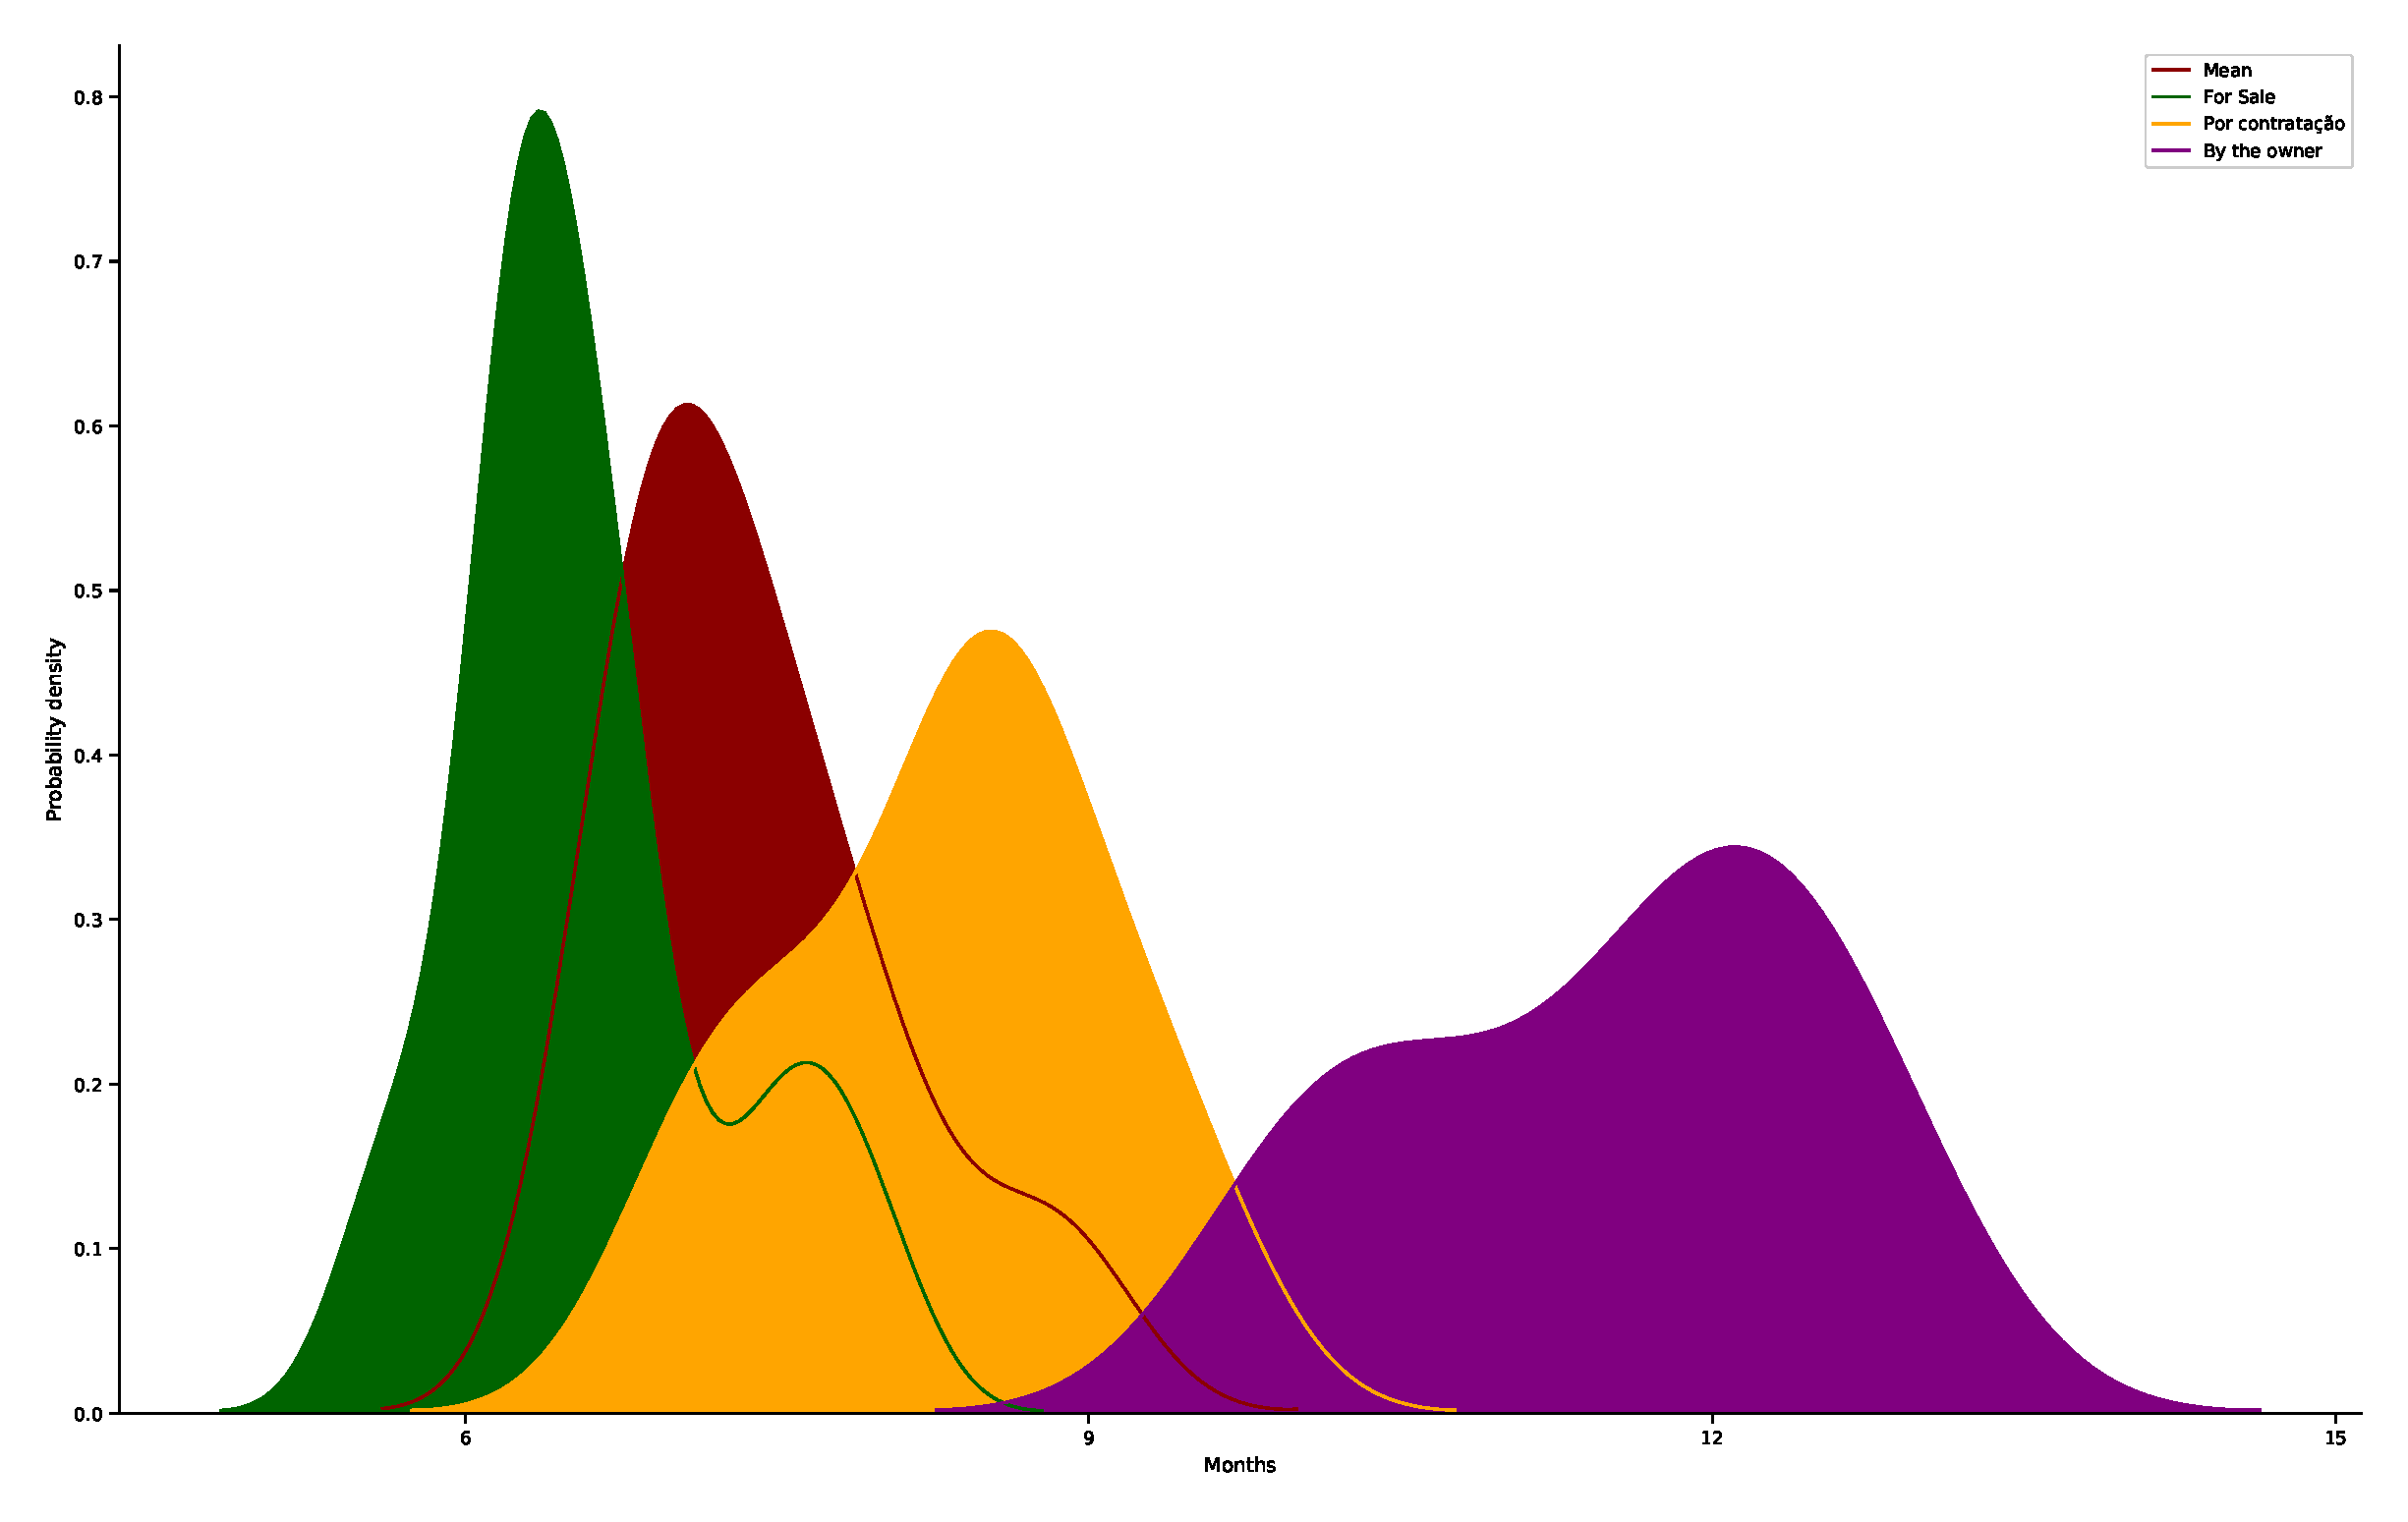
\includegraphics[height=.4\textheight]{./figs/Meses_contrucao.eps}
	\caption*{\textbf{Source:} Survey of Construction (SOC), Authors' elaboration}
\end{figure}

This procedure, however, it is not enough to determine the model order. 
Since residential investment (flow) is significantly smaller than dwelling ()existing stock), the price variation effect  is verified even
when the construction is unfinished. 
We argue that this price effect is a result of future real estate inflation.
Such dynamic would be captured by the \textbf{expected} houses' own interest rate.
However, such series does not exist. So, we use lagged houses' own interest rate as a first approximation to the expected one\footnote{
	This procedure is similar to \textcite{keynes_general_1937} ``practical theory of the future'' in which decision-making process for buying a new property depends on expectations/conventions based on past observations. 
	In summary, in the absence of a series for the expected own interest rate, the lag of this variable will be used as a proxy for the future one.
}.

In order to display the relation between lagged own interest rate and current residential investment growth rate, Figure \ref{defasagens} depicts one variable of interest against the other variable lagged according to lags that minimize the information criteria (1 and 4 respectively)\footnote{
	Similar plot can be seen in \textcite[p.~16]{girardi_autonomous_2015}.
}.
This simple procedure allows checking if there is any relationship between the expected own interest rate (in this case, lagged effective rate) and residential investment growth rate\footnote{
	In order to consider non-linearities, we presented quadratic regression between variables of interest.
}.
In the same Figure, we verify that the inverse relationship, that is, from residential investment to own interest rate, does not occur. 
The lack of relationship in the opposite direction reflects a dynamics already mentioned before.
Since residential investment (flow) is much lower than the existing stock of dwellings, it is expected that such relationship does not exist.
In summary, speculation with the dwellings stock generates inflation of these assets, which affects the construction of new houses (flow) and not the other way round\footnote{
	It is worth noting a particular aspect of house price formation: land scarcity. As a consequence, speculation with residences is, in the end, speculation with land (the only scarce resource involved in its production) and, therefore, it is relevant for speculation with the dwellings stock. 
	\textcite[p.~349, emphasis added]{leamer_housing_2007} points out this particularity as follows:
	\begin{quotation}
		It’s not the structure that has a volatile price; \textbf{it's the land}. Where there is plenty of buildable land, the response to an increase is demand for homes is mostly to build more, not to increase prices. Where there is little buildable land, the response to an increase in demand for homes is mostly a price increase, sufficient to discourage buyers enough to reequilibrate the supply and demand.
	\end{quotation}
}.


\begin{figure}
	\centering
	\caption{Dispersion between houses' own interest rate and residential investment growth: lags selected based on information criteria}
	\label{defasagens}
	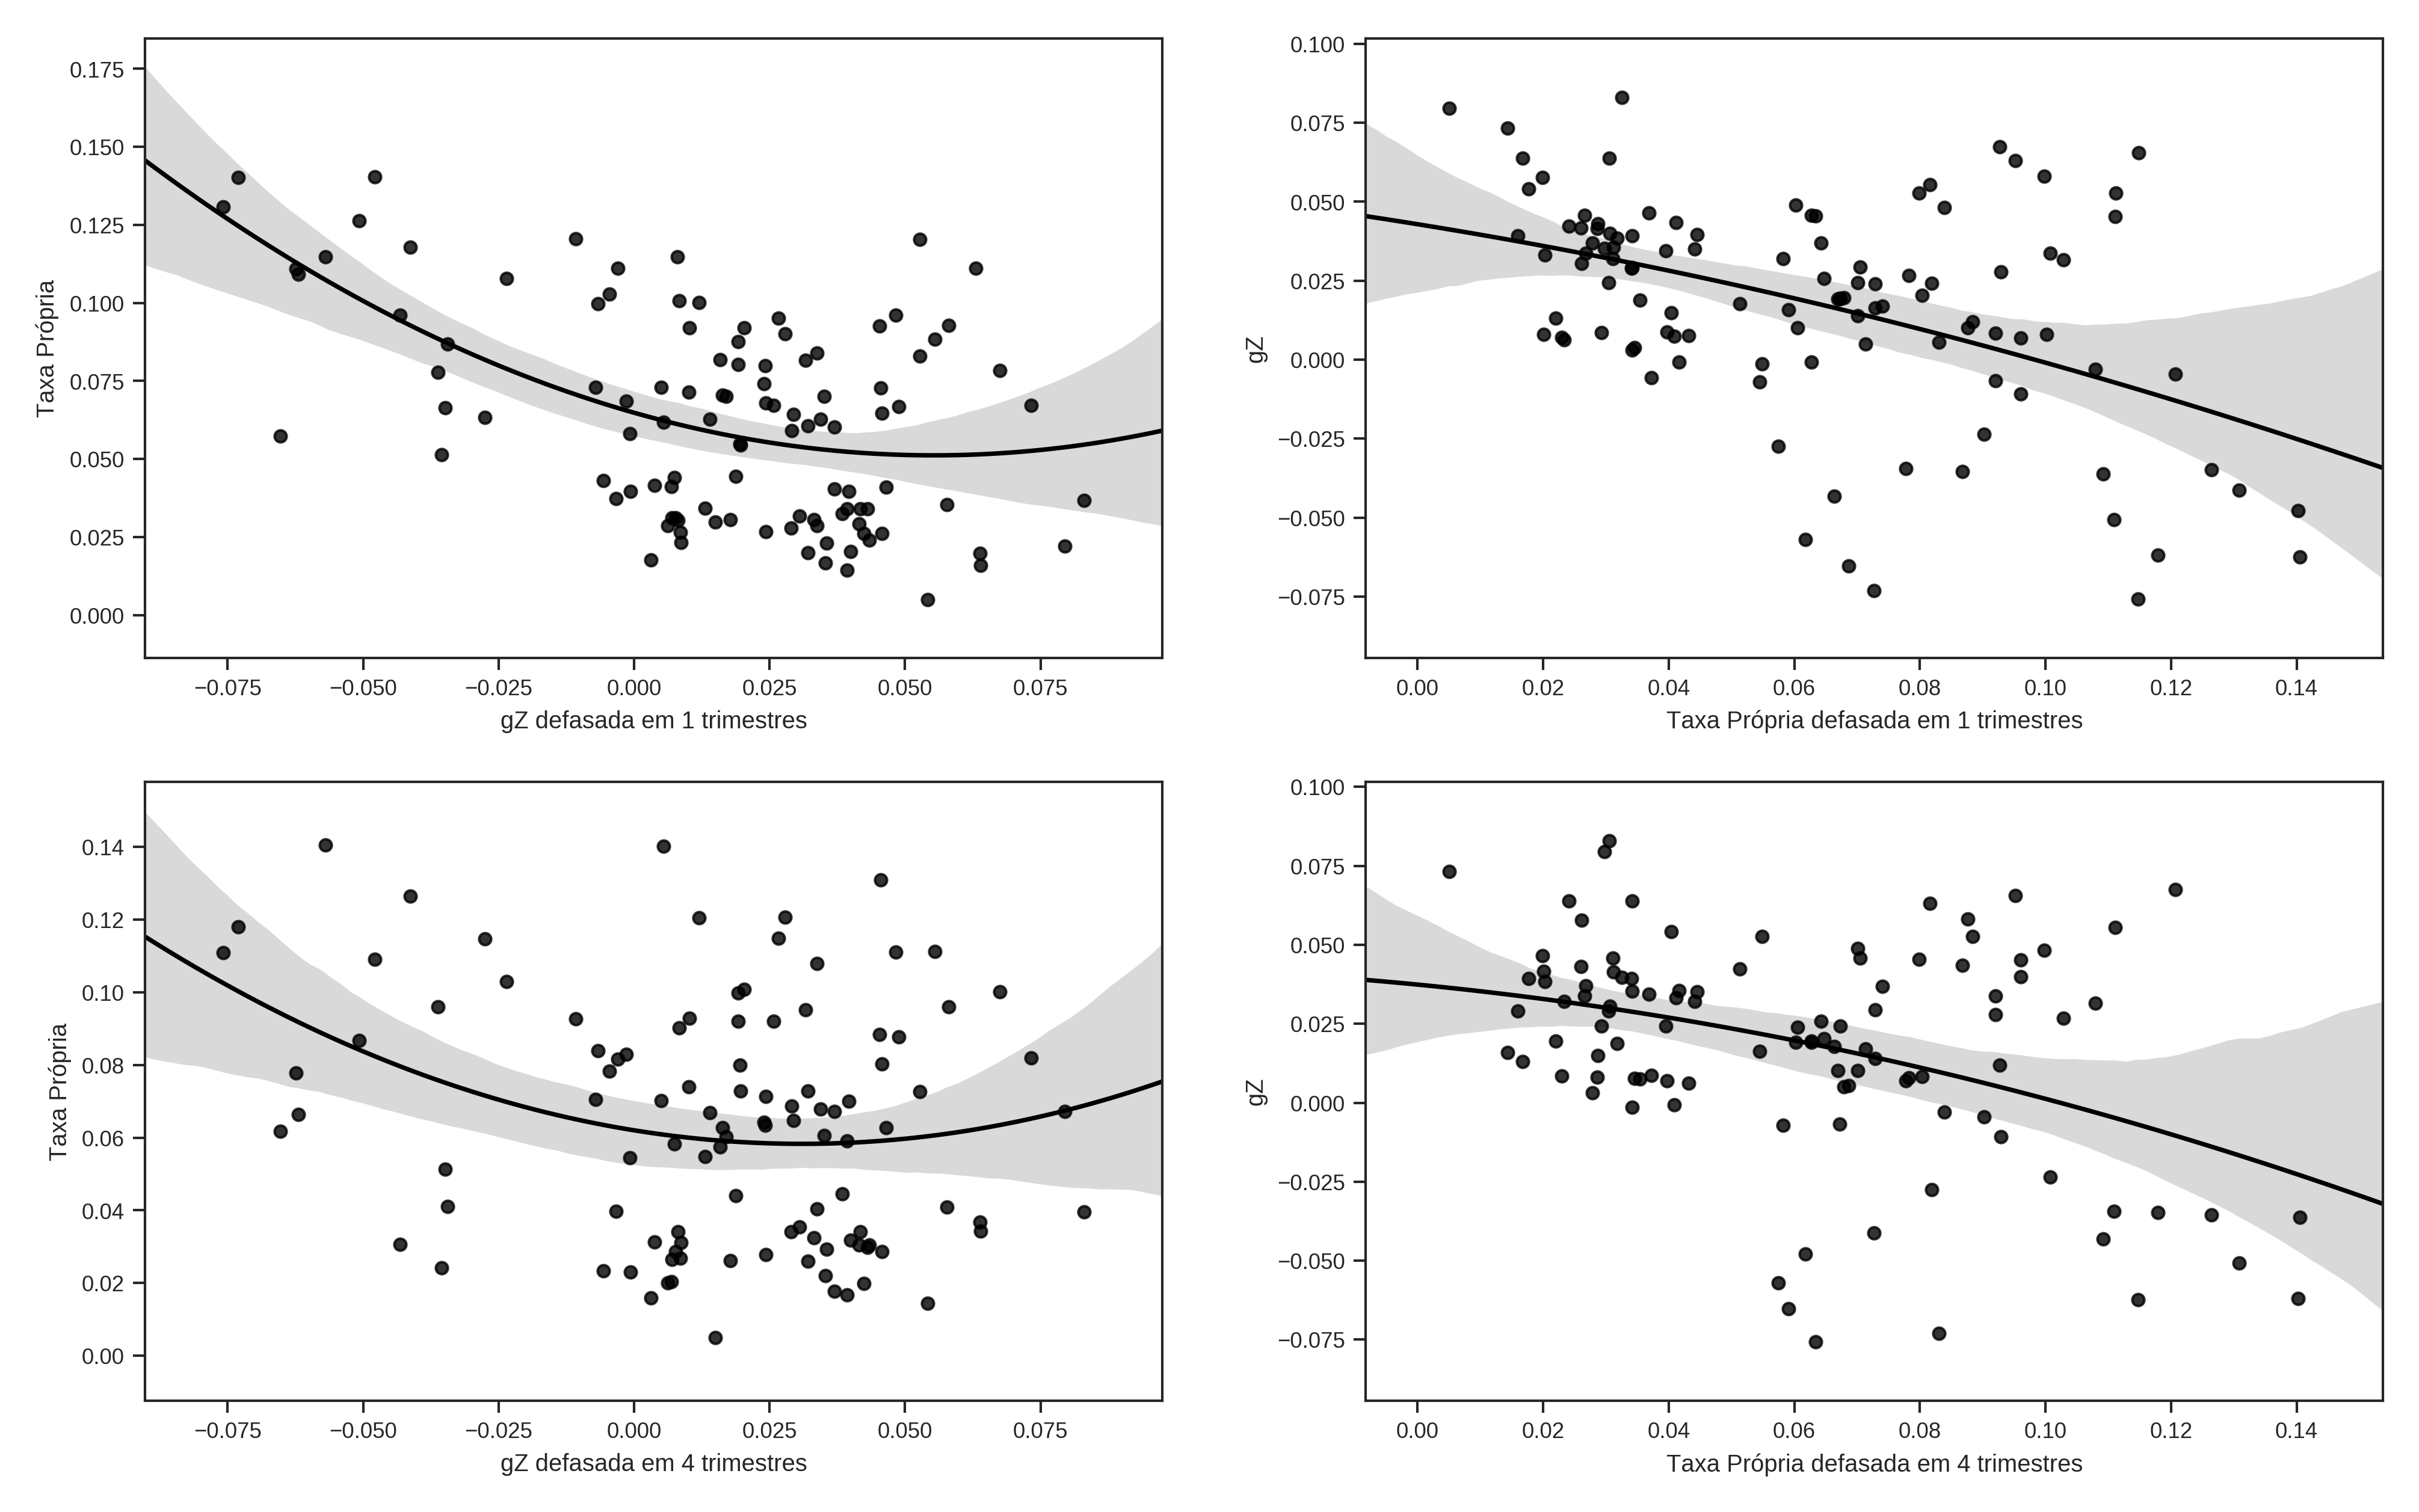
\includegraphics[height=.4\textheight]{./figs/VEC_Defasagens.eps}
	\caption*{\textbf{Source:} Authors' elaboration}
\end{figure}


From this theoretical and econometric discussion of model order specification, we estimate a VEC with four lags (see Table \ref{Estimacao})\footnote{
	In addition to being theoretically based, this lag also generates homocedastic residuals without serial auto-correlation (see Table \ref{testes_resduos} in Appendix \ref{appen:A}).
}. 
Figure \ref{residuos} displays an inspection of the residuals while Table \ref{testes_resduos} in Appendix \ref{appen:A} presents a few residual tests to check the model's specification.
On the following subsection, we analyze if our estimation supports the hypothesis presented in Table \ref{resultados_esperados} above.  



\subsection{Estimation results}\label{sec:results}

According to parameters presented in Table \ref{Estimacao}, we find statistically significant cointegration  coefficients for both equations. 
Therefore, both variables share a (negative) long-run trend (validating hypotheses 1 and 4).
The short-term relationship between $own$ and $g_{Ih}$ ($\beta_{1, is}$ coefficients) are not statistically significant at 5\%\footnote{
	The expected result (7) can also be validated from the inspection of Table \ref{Estimacao} in which only the fourth lag of own interest rate equation is statistically significant.
}.
In addition, coefficients $\gamma_{2,s}$ are negative and statistically significant at 5\%, supporting hypothesis 6 (see Table  \ref{Estimacao}). 
We also find statistically significant coefficients related to demand for properties for non-speculative reasons ($\phi_0$), validating proposition 5.
On the other hand, the error correction parameter is statistically significant only for the residential investment growth rate equation.
In this sense, $own$ is weakly exogenous compared to $g_{I_h}$ while houses' own interest rate Granger-causes $g_{I_h}$, supporting the hypothesis (2) and (3).
In conclusion, our estimation results are in line with the hypothesis presented above and can be summarized as follows: houses' own interest rate determines --- but is not determined by --- residential investment growth rate and these variables present a negative long-term relationship (are cointegrated).


\begin{table}[h!]
	\caption{Estimation parameters}
	\label{Estimacao}
\begin{threeparttable}
	\centering
	\begin{tabular}{lcccccc}
		\hline \hline
		\textbf{Equation:} $own$ & \textbf{coef} & \textbf{std err} & \textbf{z} & \textbf{P$> |$z$|$} & \textbf{[0.025} & \textbf{0.975]}  \\
		\midrule
		\textbf{$\delta_{1}$}      &   -1.632e-05  &      4.4e-05     &    -0.371  &         0.710        &       -0.000    &     6.98e-05     \\
		\textbf{$\gamma_{1,1}$ ($L_1$ $own$)} &       0.0381  &        0.111     &     0.342  &         0.732        &       -0.180    &        0.256     \\
		\textbf{$\beta_{1,1}$ ($L_1 g_{I_h}$)}           &       0.0738  &        0.083     &     0.887  &         0.375        &       -0.089    &        0.237     \\
		\textbf{$\gamma_{1,2}$ ($L_2$ $own$)} &      -0.0032  &        0.110     &    -0.029  &         0.977        &       -0.218    &        0.212     \\
		\textbf{$\beta_{1,2}$ ($L_2 g_{I_h}$)}           &       0.1115  &        0.082     &     1.366  &         0.172        &       -0.048    &        0.272     \\
		\textbf{$\gamma_{1,3}$ ($L_3$ $own$)} &       0.0757  &        0.118     &     0.642  &         0.521        &       -0.156    &        0.307     \\
		\textbf{$\beta_{1,3}$ ($L_3 g_{I_h}$)}           &       0.1080  &        0.069     &     1.563  &         0.118        &       -0.027    &        0.243     \\
		\textbf{$\gamma_{1,4}$ ($L_4$ $own$)} &       0.2649  &        0.119     &     2.230  &         0.026$^{***}$        &        0.032    &        0.498     \\
		\textbf{$\beta_{1,4}$ ($L_4 g_{I_h}$)}           &      0.0583  &        0.054     &    1.089  &         0.276        &       -0.047    &       0.163     \\
		\midrule
		\textbf{Equation:} $g_{I_h}$ & \textbf{coef} & \textbf{std err} & \textbf{z} & \textbf{P$> |$z$|$} & \textbf{[0.025} & \textbf{0.975]}  \\
		\midrule
		\textbf{$\delta_{2}$}      &      -0.0003  &     6.96e-05     &    -3.848  &         0.000$^{***}$        &       -0.000    &       -0.000     \\
		\textbf{$\gamma_{2,1}$ ($L_1$ $own$)} &      -0.1747  &        0.176     &    -0.991  &         0.322        &       -0.520    &        0.171     \\
		\textbf{$\beta_{2,1}$ ($L_2 g_{I_h}$)}           &      -0.4203  &        0.132     &    -3.191  &         0.001$^{***}$        &       -0.678    &       -0.162     \\
		\textbf{$\gamma_{2,2}$ ($L_2$ $own$)} &      -0.9997  &        0.174     &    -5.752  &         0.000$^{***}$        &       -1.340    &       -0.659     \\
		\textbf{$\beta_{2,2}$ ($L_1 g_{I_h}$)}           &      -0.4596  &        0.129     &    -3.555  &         0.000$^{***}$        &       -0.713    &       -0.206     \\
		\textbf{$\gamma_{2,3}$ ($L_3$ $own$)} &      -0.5863  &        0.187     &    -3.137  &         0.002$^{***}$        &       -0.953    &       -0.220     \\
		\textbf{$\beta_{2,3}$ ($L_3 g_{I_h}$)}           &      -0.1991  &        0.109     &    -1.820  &         0.069*        &       -0.414    &        0.015     \\
		\textbf{$\gamma_{2,4}$ ($L_4$ $own$)} &      -0.5350  &        0.188     &    -2.844  &         0.004$^{***}$        &       -0.904    &       -0.166     \\
		\textbf{$\beta_{2,4}$ ($L_4 g_{I_h}$)}           &      -0.2444  &        0.085     &    -2.885  &         0.004$^{***}$        &       -0.411    &       -0.078     \\
		\midrule
		\textbf{Error correction} & \textbf{coef} & \textbf{std err} & \textbf{z} & \textbf{P$> |$z$|$} & \textbf{[0.025} & \textbf{0.975]}  \\
		\midrule
		\textbf{$\alpha_1$} &      -0.0232  &        0.071     &    -0.328  &         0.743        &       -0.162    &        0.116     \\
		\textbf{$\alpha_2$} &      -0.4245  &        0.112     &    -3.784  &         0.000$^{***}$        &       -0.644    &       -0.205     \\
		\midrule
		\textbf{Cointegration relationship} & \textbf{coef} & \textbf{std err} & \textbf{z} & \textbf{P$> |$z$|$} & \textbf{[0.025} & \textbf{0.975]}  \\
		\midrule
		\textbf{$\phi_{1,1}$} &       1.0000  &            0     &         0  &         0.000$^{***}$        &        1.000    &        1.000     \\
		\textbf{$\phi_{1,2}$} &       1.2835  &        0.149     &     8.599  &         0.000$^{***}$        &        0.991    &        1.576     \\
		\textbf{$\phi_0$}  &      -0.1131  &        0.009     &   -12.528  &         0.000$^{**}$       &       -0.131    &       -0.095     \\
		\hline
		\hline
	\end{tabular}
	%\caption{Det. terms outside the coint. relation & lagged endog. parameters for equation $own$}
\footnotesize{(*) Statistically significant at 10\%; (**) Statistically significant at 5\%; (***) Statistically significant at 1\%.}
\end{threeparttable}
	\caption*{\textbf{Source:} Authors' elaboration}
\end{table}

\begin{figure}
	\centering
	\caption{Inspection of estimation residuals}
	\label{residuos}
	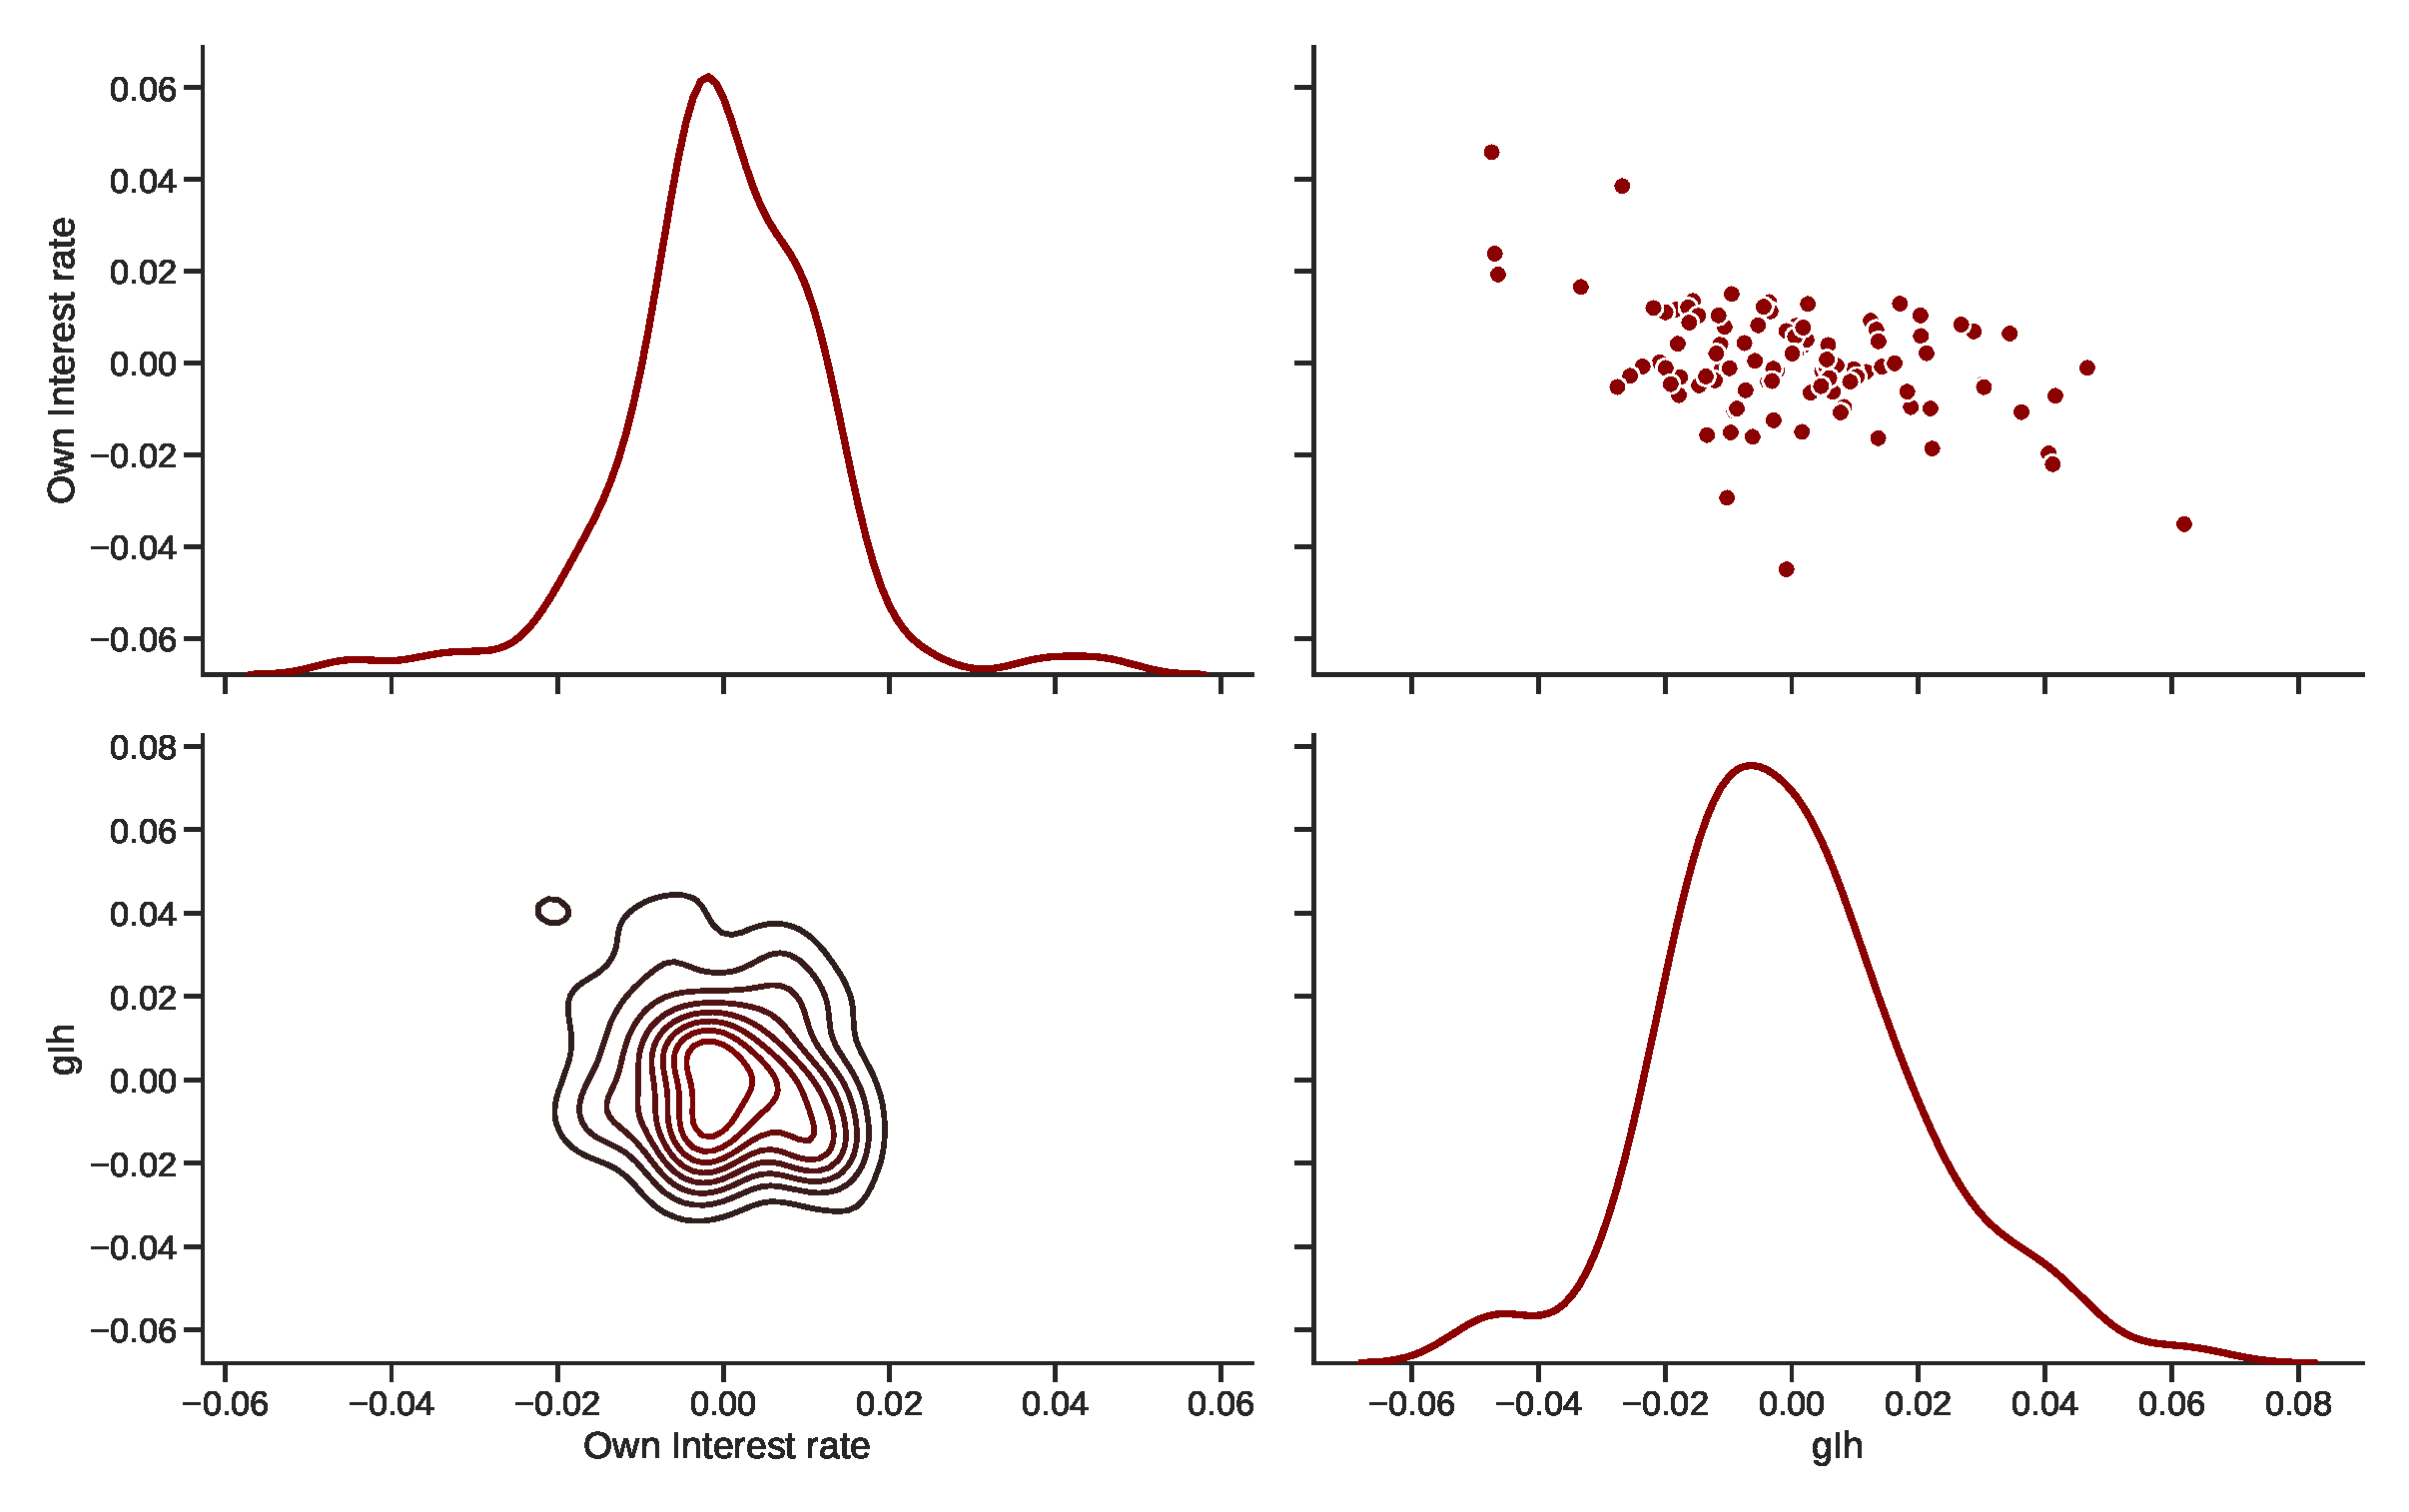
\includegraphics[height=.4\textheight]{./figs/Residuals_4VECM.eps}
	\caption*{\textbf{Source:} Authors' elaboration}
\end{figure}


Figure \ref{fevd} display the forescas error variance decomposition (FEVD) which reports houses own interest rate in describing residential investment growth rate dynamics\footnote{
	It is important to note that the number of variables (two) used generates similar  of a Structural VEC, which means that Choleski's decomposition
	is sufficient to analyze the (orthogonalized) impulse response function.
}.
We report that own interest rate has  depicted  $g_{Ih}$ --- while the reverse is not valid --- since the first quarter.
In addition, we find that such contribution is growing and greater than 50\% beyond the third quarter.
Therefore, houses' own interest rate is explained mainly by itself and explains $g_{I_h}$ considerably.


\begin{figure}[H]
	\centering
	\caption{Forecast error variance decomposition (FEVD)}
	\label{fevd}
	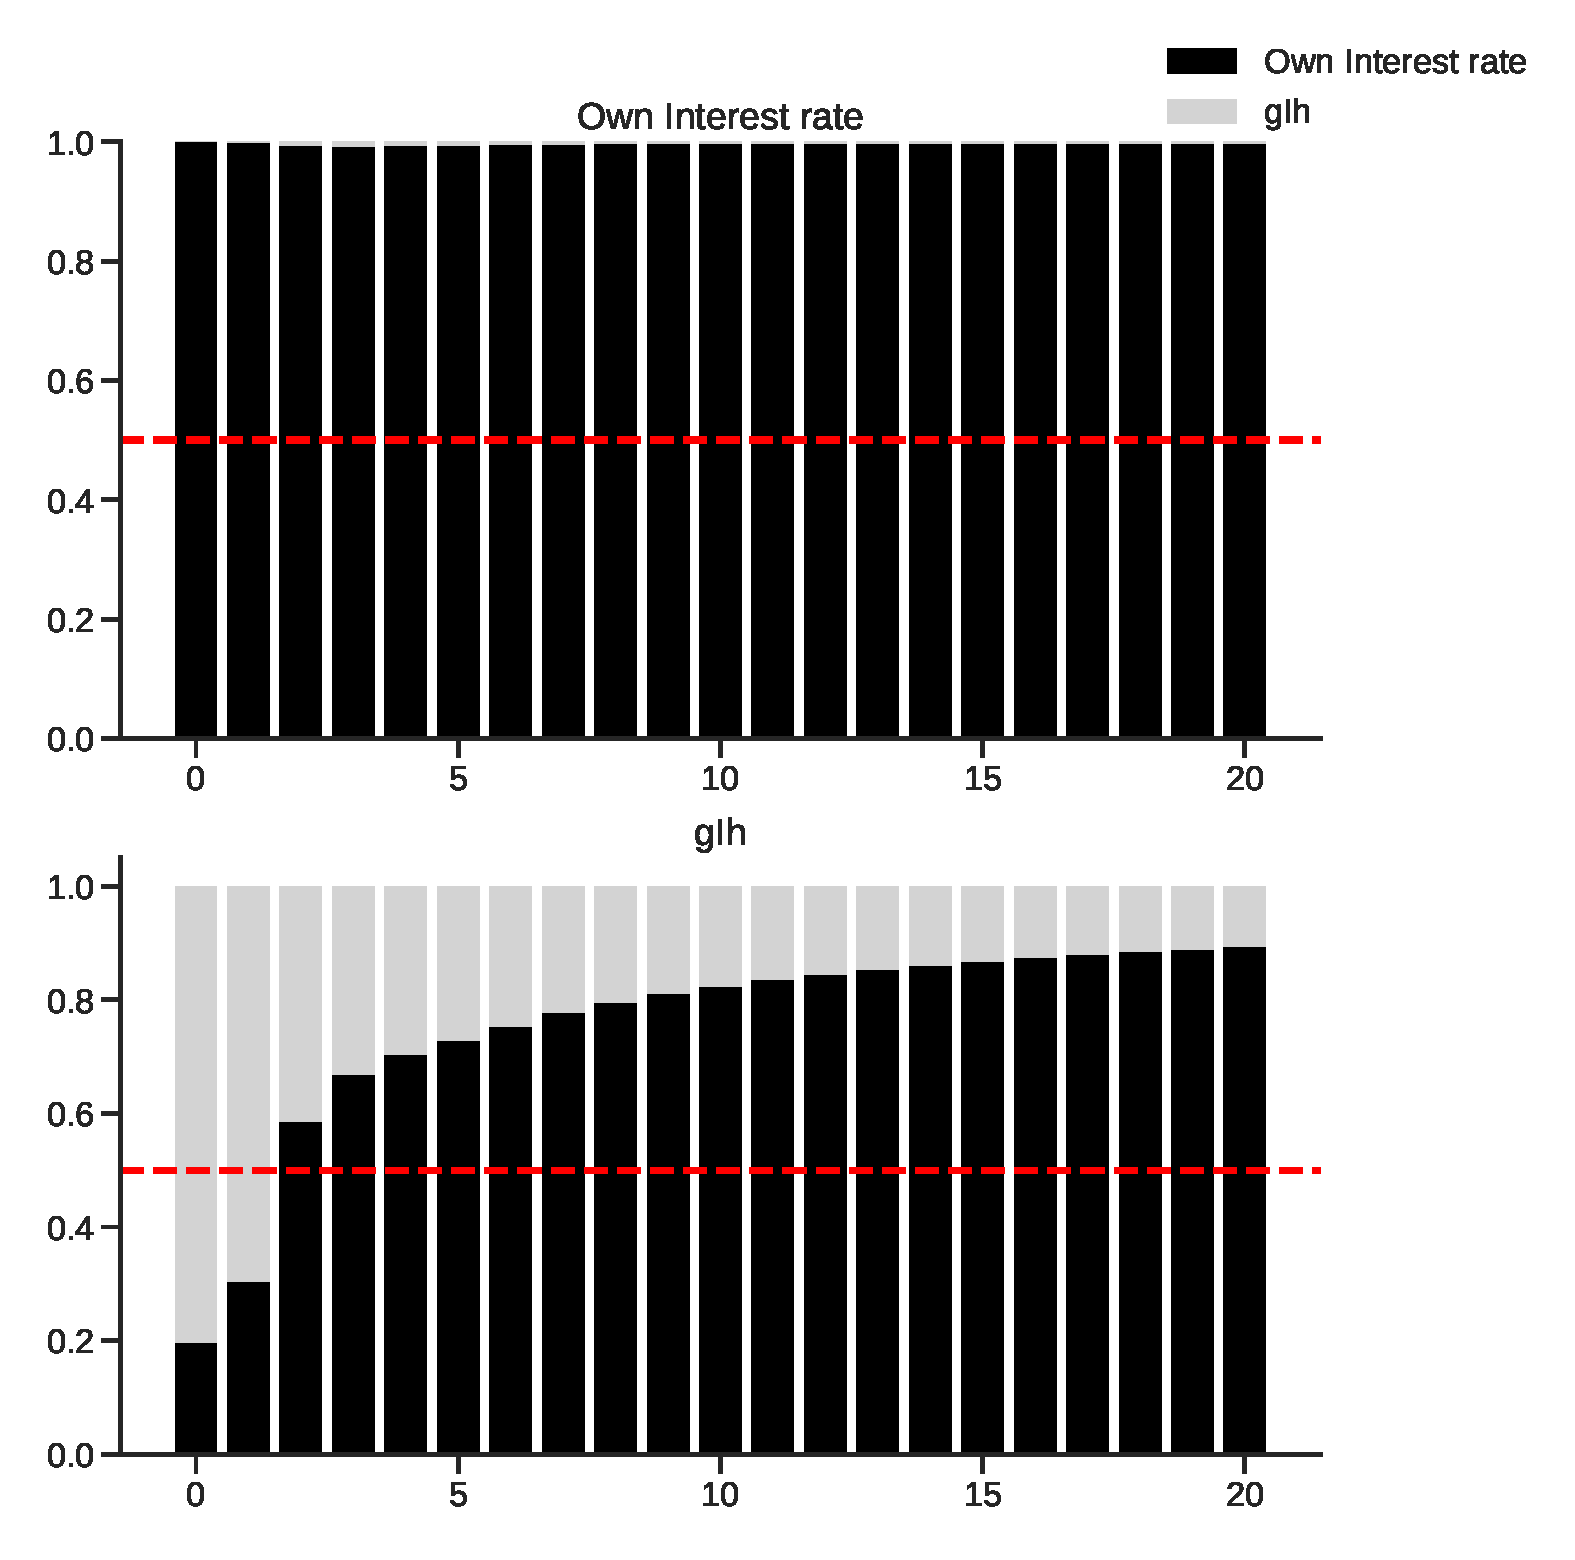
\includegraphics[height=.4\textheight]{./figs/FEVD_VECMpython_TxPropria.eps}
	\caption*{\textbf{Source:} Authors' elaboration}
\end{figure}

Next, we analyze the orthoganilized impulse response function (Figure \ref{irf}).
In summary, we report a stable system since the increase in $g_{I_h}$ on itself are dampened over time while equivalent shock on own interest rate has a non-explosive permanent effect.
On the other hand, an increase in $g_{I_h}$ has a null effect over $own$.
The most relevant result reported in Figure \ref{irf} is the considerable and lasting negative effect due to an increase in own interest rate over $g_{I_h}$, validating \textcite{teixeira_crescimento_2015} proposition.
In short, our results shows that an increase in mortgage interest rate (equivalent to an increase in houses' own interest rate) has a negative and persistent effect on residential investment growth rate while an increase in real estate inflation  has an opposite effect.

\begin{figure}[H]
	\centering
	\caption{Orthogonalized Impulse Response Function}
	\label{irf}
	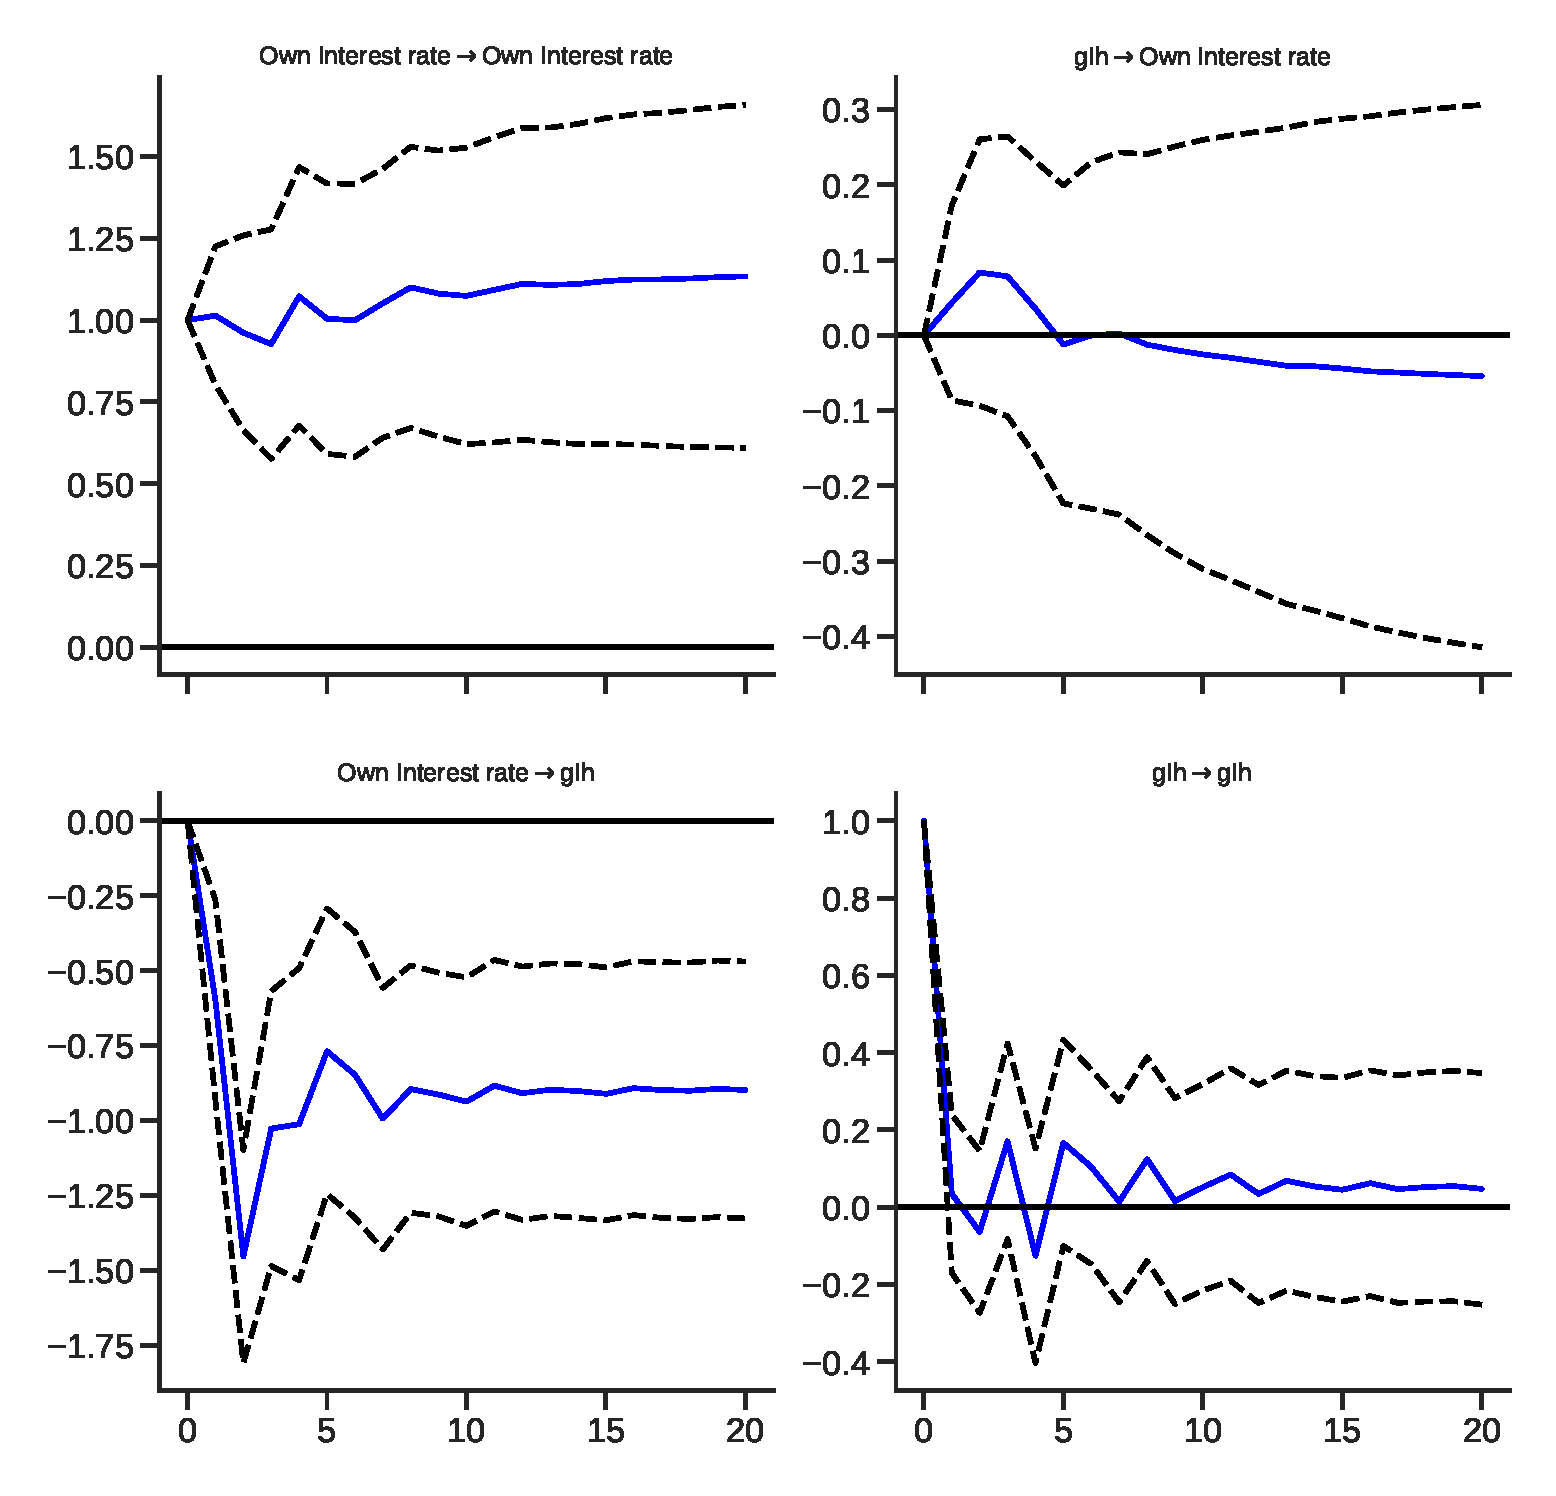
\includegraphics[height=.4\textheight]{./figs/Impulse_VECM.eps}
	\caption*{\textbf{Source:} Authors' elaboration}
\end{figure}

In summary, our estimation reports that houses' own interest rate has a prominent role in describing residential investment growth rate dynamics. 
It is worth noting that despite the amplitude of VEC order, the estimated model is quite parsimonious in terms of the number of variables.
Thus, considering its parsimony and robustness, we conclude that our estimation depicts residential investment growth rate satisfactorily.
On the following section we present some concluding remarks.







